\section{Analysis}

\begin{frame}{Value Function}
    \begin{figure}
        \centering
        \begin{subfigure}{0.33\textwidth}
            \centering
            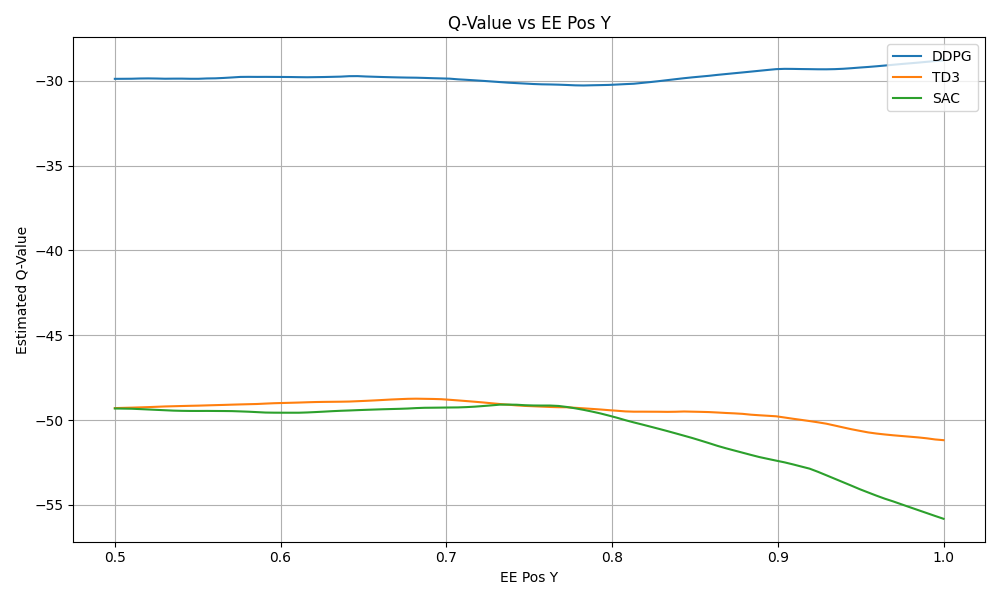
\includegraphics[width=0.75\textwidth]{FetchReach-v3_q_value_obs_EE_Pos_Y.png}
            \caption{End Effector Position (y component)}
        \end{subfigure}
        \begin{subfigure}{0.33\textwidth}
            \centering
            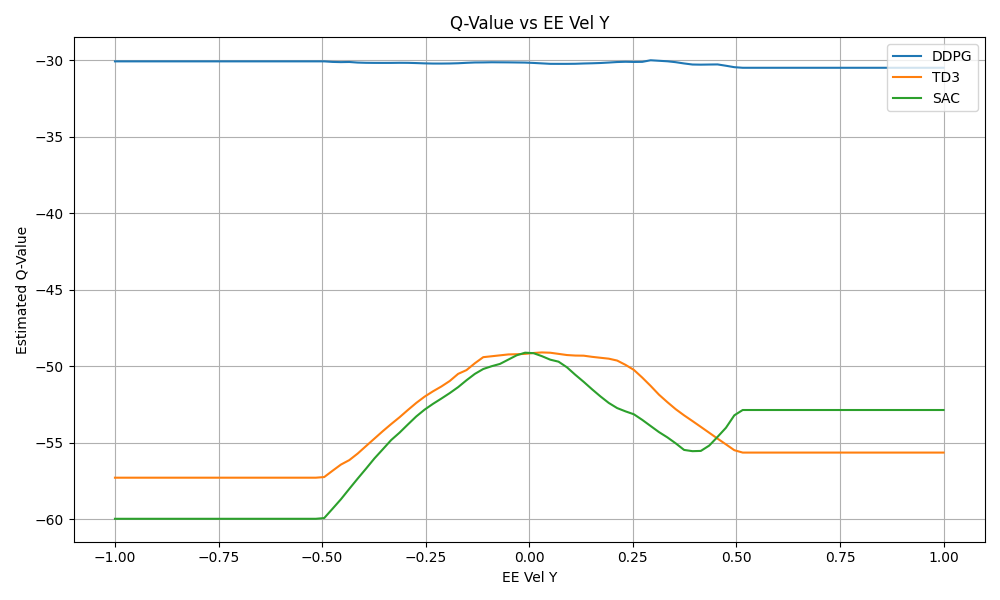
\includegraphics[width=0.75\textwidth]{FetchReach-v3_q_value_obs_EE_Vel_Y.png}
            \caption{End Effector Velocity (y component)}
        \end{subfigure}
        \begin{subfigure}{0.33\textwidth}
            \centering
            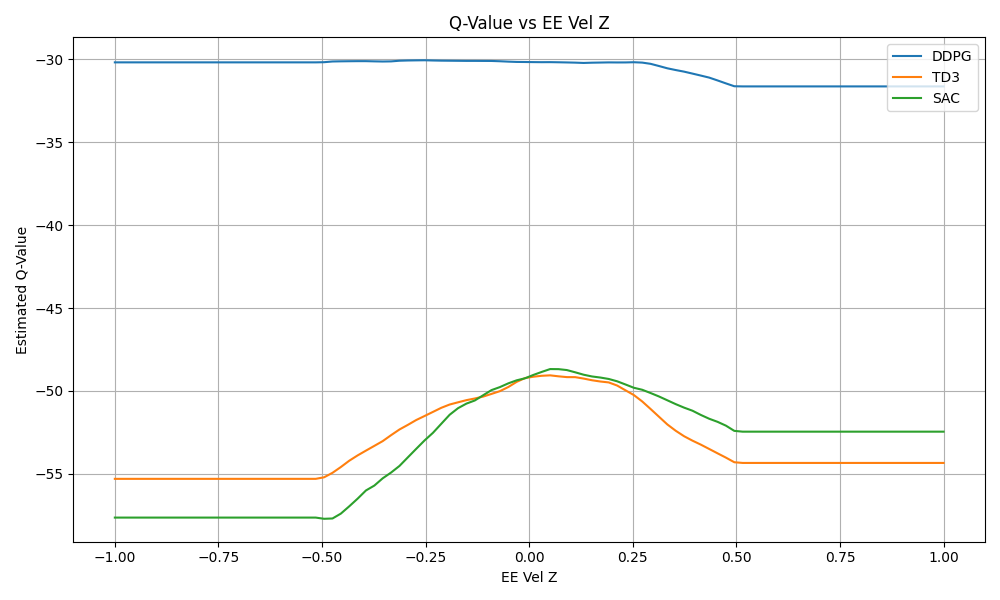
\includegraphics[width=0.75\textwidth]{FetchReach-v3_q_value_obs_EE_Vel_Z.png}
            \caption{End Effector Velocity (z component)}
        \end{subfigure}
        \begin{subfigure}{0.33\textwidth}
            \centering
            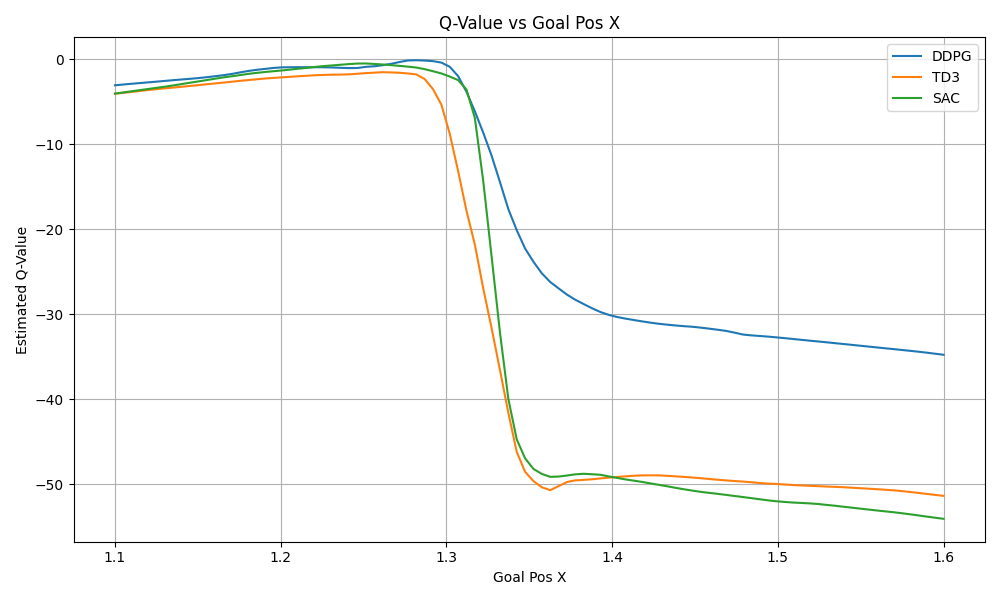
\includegraphics[width=0.75\textwidth]{FetchReach-v3_q_value_goal_Goal_Pos_X.png}
            \caption{Goal Position (x component)}
        \end{subfigure}
        \caption{Variation in Q-Value Estimates\footnote{Note that the True Q-Values cannot be found since the environment does not allow changing the initial or current state. The only way of manipulating the state is by performing actions.} along different observation dimensions. Initial EE Position = $[1.34, 0.75, 0.53]$, Goal Position = $[1.40, 0.75, 0.60]$, Velocities assumed to be zero.}
    \end{figure}
\end{frame}

\begin{frame}{Policy Function}
    \begin{figure}
        \centering
        \begin{subfigure}{0.33\textwidth}
            \centering
            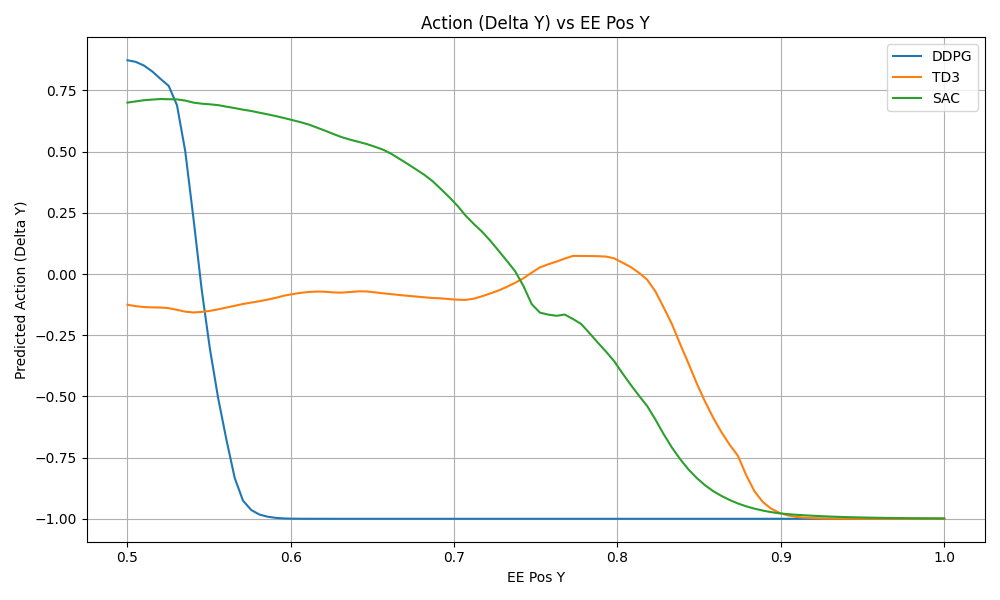
\includegraphics[width=0.75\textwidth]{FetchReach-v3_action_obs_EE_Pos_Y_vs_Delta_Y}
            \caption{End Effector Position (y component)}
        \end{subfigure}
        \begin{subfigure}{0.33\textwidth}
            \centering
            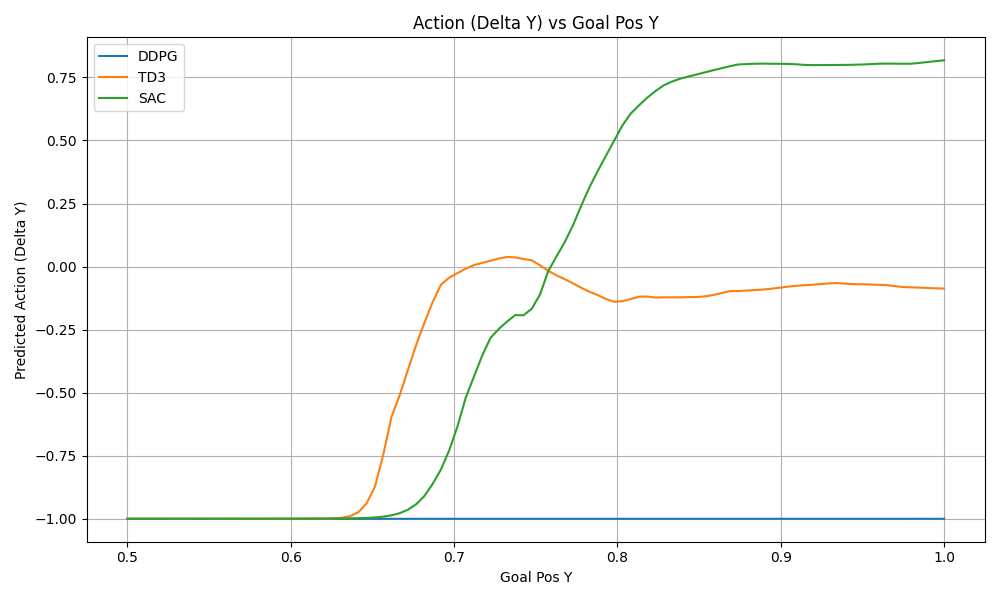
\includegraphics[width=0.75\textwidth]{FetchReach-v3_action_goal_Goal_Pos_Y_vs_Delta_Y.png}
            \caption{Goal Position (y component)}
        \end{subfigure}
        \begin{subfigure}{0.33\textwidth}
            \centering
            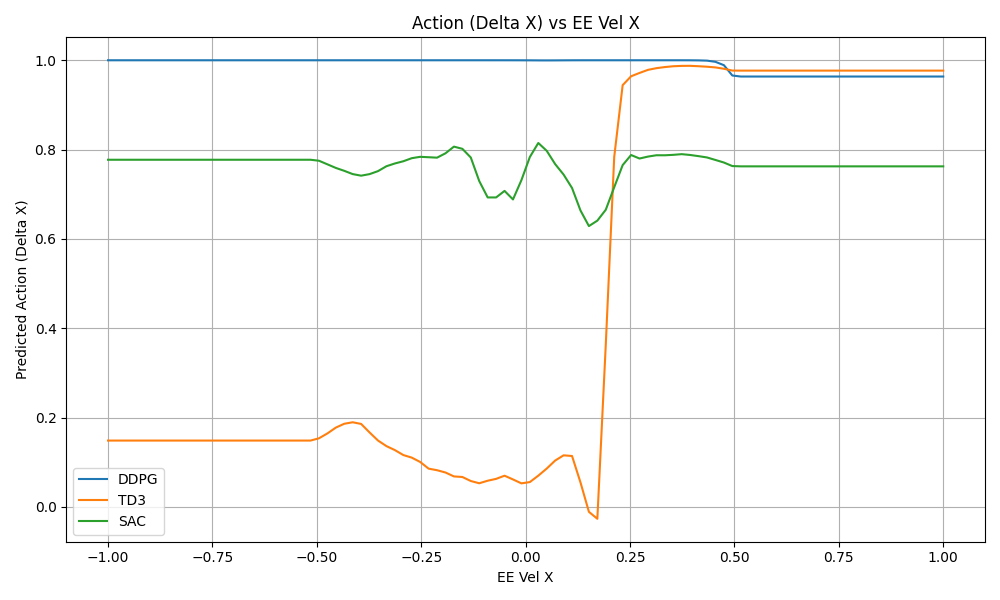
\includegraphics[width=0.75\textwidth]{FetchReach-v3_action_obs_EE_Vel_X_vs_Delta_X.png}
            \caption{End Effector Velocity (x component)}
        \end{subfigure}
        \caption{Variation in Learned Policy (in the same spatial dimension) along different observation dimensions. Initial EE Position = $[1.34, 0.75, 0.53]$, Goal Position = $[1.40, 0.75, 0.60]$, Velocities assumed to be zero.}
    \end{figure}
\end{frame}

\begin{frame}{Simulation}
    Simulation of the agent trained on the FetchReach environment can be found at \url{https://drive.google.com/file/d/13NJmlQaMdkiZFKCaScmR6k1ZMuZ1bMqM/}.
\end{frame}

\begin{frame}{Conclusion}
    \begin{itemize}
        \item Q-Value Overestimation was observed with DDPG, as noted in literature.
        \item SAC led to better estimates in both value and policy, while TD3 resulted in only better value estimates.
        \item The networks tend to learn sigmoid like curves over quadratic like curves, contrary to our expectation.
        \item Transfer learning can be beneficial for training on the FetchPush environment. The agent can learn to utilize the existing knowledge, of moving to the initial position of the block, for the stated objective of displacing the block.
        \item Alternatively, auxillary rewards, such as for moving the gripper to the initial position of the block, can be helpful for learning the `first steps'.
    \end{itemize}
\end{frame}
